\documentclass[aspectratio=169, xcolor=dvipsnames]{beamer}

% --- Theme Setup ---
\usetheme{Madrid}
\usecolortheme{default}

% --- Packages ---
\usepackage{graphicx}
\usepackage{xcolor}
\usepackage{booktabs}
\usepackage{hyperref}
\usepackage{adjustbox}
\usepackage{amssymb}
\usepackage{amsmath}
\usepackage{listings}
\usepackage{tabularx}

\lstset{
  basicstyle=\ttfamily\small,
  keywordstyle=\color{blue}\bfseries,
  stringstyle=\color{red},
  showstringspaces=false,
  breaklines=true
}

% --- Title Information ---
\title{Module 08}
\subtitle{Introduction to SQL/1}
\author{Milav Dabgar}
\institute{www.milav.in}
\date{\today}

\begin{document}

% Title Slide
\begin{frame}
    \titlepage
\end{frame}

\begin{frame}{Module Recap}
    \begin{itemize}
        \item Introduced relational algebra
        \item Familiarized with the operators of relational algebra
    \end{itemize}
\end{frame}

\begin{frame}{Module Objectives}
    \begin{itemize}
        \item To understand relational query language
        \item To understand data definition and basic query structure
    \end{itemize}
\end{frame}

\begin{frame}{Module Outline}
    \begin{itemize}
        \item History of SQL
        \item Data Definition Language (DDL)
        \item Data Manipulation Language (DML): Query Structure
    \end{itemize}
\end{frame}

\section{History of SQL}

\begin{frame}
  \vfill
  \centering
  \begin{beamercolorbox}[sep=8pt,center,shadow=true,rounded=true]{title}
    \usebeamerfont{title}History of SQL\par%
  \end{beamercolorbox}
  \vfill
\end{frame}

\begin{frame}{History of Query Language}
    \begin{itemize}
        \item IBM developed Structured English Query Language (\textbf{SEQUEL}) as part of System R project. Renamed Structured Query Language (SQL; pronounced still as SEQUEL)
        \item ANSI and ISO standard SQL:
    \end{itemize}
    \vspace{0.5em}
    \begin{center}
        \begin{adjustbox}{max width=\textwidth}
        \begin{tabular}{|l|p{12cm}|}
        \hline
        \textbf{SQL-86} & First formalized by ANSI \\ \hline
        \textbf{SQL-89} & + Integrity Constraints \\ \hline
        \textbf{SQL-92} & Major revision (ISO/IEC 9075 standard), De-facto Industry Standard \\ \hline
        \textbf{SQL:1999} & + Regular Expression Matching, Recursive Queries, Triggers, Support for Procedural and Control Flow Statements, Nonscalar types (Arrays), and Some OO features, Embedding SQL in Java (SQL/OLB), and Embedding Java in SQL (SQL/JRT) \\ \hline
        \textbf{SQL:2003} & + XML features (SQL/XML), Window Functions, Standardized Sequences, and Columns with Auto-generated Values \\ \hline
        \end{tabular}
        \end{adjustbox}
    \end{center}
\end{frame}

\begin{frame}{History of Query Language (cont.)}
    \begin{center}
        \begin{adjustbox}{max width=\textwidth}
        \begin{tabular}{|l|p{12cm}|}
        \hline
        \textbf{SQL:2006} & + Ways of importing and storing XML data in an SQL database, manipulating it, and publishing both XML and conventional SQL-data in XML form \\ \hline
        \textbf{SQL:2008} & Legalizes \texttt{ORDER BY} outside Cursor Definitions + \texttt{INSTEAD OF} Triggers, \texttt{TRUNCATE} Statement, and \texttt{FETCH} Clause \\ \hline
        \textbf{SQL:2011} & + Temporal Data (\texttt{PERIOD FOR}), Enhancements for Window Functions and \texttt{FETCH} Clause \\ \hline
        \textbf{SQL:2016} & + Row Pattern Matching, Polymorphic Table Functions, and JSON \\ \hline
        \textbf{SQL:2019} & + Multidimensional Arrays (MDarray type and operators) \\ \hline
        \end{tabular}
        \end{adjustbox}
    \end{center}
\end{frame}

\begin{frame}{History of Query Language (2): Compliance}
    \begin{itemize}
        \item SQL is the de facto industry standard today for relational or structured data systems
        \item Commercial systems as well as open systems may be fully or partially compliant to one or more standards from SQL-92 onward
        \item Not all examples here may work on your particular system. Check your system's SQL documentation!
    \end{itemize}
\end{frame}

\begin{frame}{History of Query Language (3): Alternatives}
    \begin{itemize}
        \item There aren't any alternatives to SQL for speaking to relational databases (that is, SQL as a protocol), but there are many alternatives to writing SQL in the applications
        \item These alternatives have been implemented in the form of frontends for working with relational databases.
        \item Some examples of a frontend include:
        \begin{itemize}
            \item \textbf{SchemeQL} and \textbf{CLSQL}, which are probably the most flexible, owing to their Lisp heritage
            \item \textbf{LINQ} (in .Net)
            \item \textbf{ScalaQL} and \textbf{ScalaQuery} (in Scala)
            \item \textbf{SqlStatement}, \textbf{ActiveRecord} and many others in Ruby
            \item \textbf{HaskellDB}
            \item \dots the list goes on for many other languages.
        \end{itemize}
    \end{itemize}
\end{frame}

\begin{frame}{History of Query Language (4): Derivatives}
    \begin{itemize}
        \item There are several query languages that are derived from or inspired by SQL. Of these, the most popular and effective is \textbf{SPARQL}.
        \item \textbf{SPARQL} (pronounced \textit{sparkle}, a recursive acronym for SPARQL Protocol and RDF Query Language) is an RDF query language
        \begin{itemize}
            \item[$\triangleright$] A semantic query language for databases - able to retrieve and manipulate data stored in Resource Description Framework (RDF) format.
            \item[$\triangleright$] It has been standardized by the W3C Consortium as key technology of the semantic web
            \item[$\triangleright$] Versions: SPARQL 1.0 (January 2008) and SPARQL 1.1 (March, 2013)
            \item[$\triangleright$] Used as the query languages for several NoSQL systems - particularly the Graph Databases that use RDF as store
        \end{itemize}
    \end{itemize}
\end{frame}

\section{Data Definition Language (DDL)}

\begin{frame}
  \vfill
  \centering
  \begin{beamercolorbox}[sep=8pt,center,shadow=true,rounded=true]{title}
    \usebeamerfont{title}Data Definition Language (DDL)\par%
  \end{beamercolorbox}
  \vfill
\end{frame}

\begin{frame}{Data Definition Language (DDL)}
    The SQL data-definition language (DDL) allows the specification of information about relations, including:
    \begin{itemize}
        \item The Schema for each Relation
        \item The Domain of values associated with each Attribute
        \item Integrity Constraints
        \item And also other information such as:
        \begin{itemize}
            \item The set of Indices to be maintained for each relation
            \item Security and Authorization information for each relation
            \item The Physical Storage Structure of each relation on disk
        \end{itemize}
    \end{itemize}
\end{frame}

\begin{frame}{Domain Types in SQL}
    \begin{itemize}
        \item \texttt{char(n)}: Fixed length character string, with user-specified length $n$
        \item \texttt{varchar(n)}: Variable length character strings, with user-specified maximum length $n$
        \item \texttt{int}: Integer (a finite subset of the integers that is machine-dependent)
        \item \texttt{smallint(n)}: Small integer (a machine-dependent subset of the integer domain type)
        \item \texttt{numeric(p, d)}: Fixed point number, with user-specified precision of $p$ digits, with $d$ digits to the right of decimal point. (e.g., \texttt{numeric(3, 1)} allows $44.5$ but not $444.5$ or $0.32$)
        \item \texttt{real, double precision}: Floating point and double-precision floating point numbers
        \item \texttt{float(n)}: Floating point number, with user-specified precision of at least $n$ digits
    \end{itemize}
\end{frame}

\begin{frame}{Schema Diagram for University Database}
    \begin{center}
        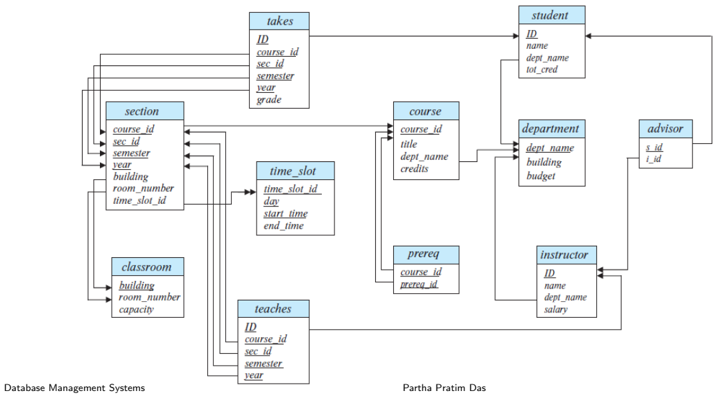
\includegraphics[height=0.8\textheight, width=\textwidth, keepaspectratio]{../Lecture 2.3_artifacts/image_000014_94c8d75bd0499771257241e28b4d6461a7881c3575c1aef605e9a8d26650b0fd.png}
    \end{center}
\end{frame}

\begin{frame}[fragile]{Create Table Construct}
    \begin{itemize}
        \item An SQL relation is defined using the \texttt{create table} command:
    \end{itemize}
    \begin{lstlisting}[language=SQL]
create table r (
    A1 D1,
    A2 D2,
    ...,
    An Dn,
    (integrity-constraint_1),
    ...,
    (integrity-constraint_k)
);
    \end{lstlisting}
    \begin{itemize}
        \item \texttt{r} is the name of the relation
        \item each \texttt{A\_i} is an attribute name in the schema of relation \texttt{r}
        \item \texttt{D\_i} is the data type of values in the domain of attribute \texttt{A\_i}
    \end{itemize}
\end{frame}

\begin{frame}[fragile]{Create Table Construct (2)}
    \begin{lstlisting}[language=SQL]
create table instructor (
    ID          char(5),
    name        varchar(20),
    dept_name   varchar(20),
    salary      numeric(8,2)
);
    \end{lstlisting}
\end{frame}

\begin{frame}[fragile]{Create Table Construct (3): Integrity Constraints}
    \begin{itemize}
        \item \texttt{not null}
        \item \texttt{primary key ($A_1, \dots, A_n$)}
        \item \texttt{foreign key ($A_m, \dots, A_n$) references r}
    \end{itemize}
    
    \begin{lstlisting}[language=SQL]
create table instructor (
    ID          char(5),
    name        varchar(20) not null,
    dept_name   varchar(20),
    salary      numeric(8,2),
    primary key (ID),
    foreign key (dept_name) references department
);
    \end{lstlisting}
    \vspace{0.5em}
    \textit{Primary key declaration on an attribute automatically ensures \texttt{not null}}
\end{frame}

\begin{frame}{University Schema}
    \begin{center}
        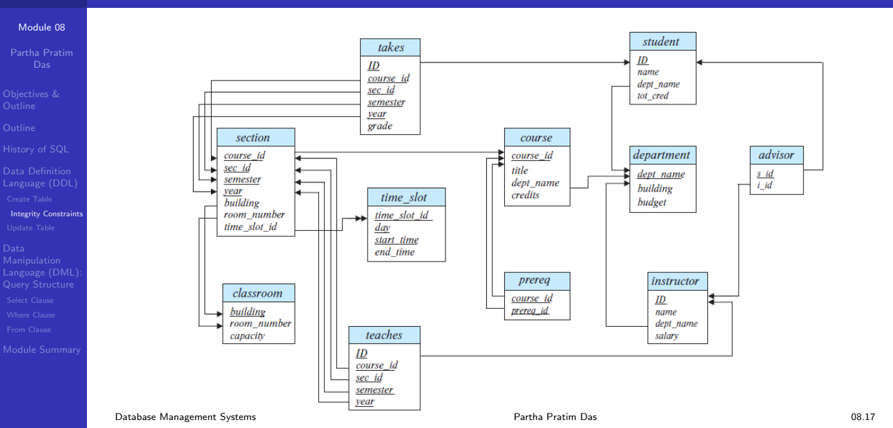
\includegraphics[height=0.8\textheight, width=\textwidth, keepaspectratio]{../Lecture 2.3_artifacts/image_000021_c9afd06ce7ef2f0a1b43dc5d88e03116f2179e0767d6ba8b8ce1ccf7ddb512b4.png}
    \end{center}
\end{frame}

\begin{frame}[fragile]{Create Table Construct (4): More Relations}
    \begin{lstlisting}[language=SQL, basicstyle=\ttfamily\scriptsize]
create table student (
    ID          varchar(5),
    name        varchar(20) not null,
    dept_name   varchar(20),
    tot_cred    numeric(3, 0),
    primary key (ID),
    foreign key (dept_name) references department
);

create table takes (
    ID          varchar(5),
    course_id   varchar(8),
    sec_id      varchar(8),
    semester    varchar(6),
    year        numeric(4, 0),
    grade       varchar(2),
    primary key (ID, course_id, sec_id, semester, year),
    foreign key (ID) references student,
    foreign key (course_id, sec_id, semester, year) references section
);
    \end{lstlisting}
    \flushleft \scriptsize \textit{Note: \texttt{sec\_id} can be dropped from primary key above, to ensure a student cannot be registered for two sections of the same course in the same semester}
\end{frame}

\begin{frame}[fragile]{Update Tables}
    \begin{itemize}
        \item \textbf{Insert (DML command)}
        \begin{lstlisting}[language=SQL, basicstyle=\ttfamily\scriptsize]
insert into instructor values ('10211', 'Smith', 'Biology', 66000);
        \end{lstlisting}
        \item \textbf{Delete (DML command)} : Remove all tuples from the student relation
        \begin{lstlisting}[language=SQL, basicstyle=\ttfamily\scriptsize]
delete from student;
        \end{lstlisting}
        \item \textbf{Drop Table (DDL command)}
        \begin{lstlisting}[language=SQL, basicstyle=\ttfamily\scriptsize]
drop table r;
        \end{lstlisting}
        \item \textbf{Alter (DDL command)}
        \begin{lstlisting}[language=SQL, basicstyle=\ttfamily\scriptsize]
alter table r add A D;
        \end{lstlisting}
        \begin{itemize}
            \item[$\triangleright$] Where \texttt{A} is the attribute name and \texttt{D} is the domain
            \item[$\triangleright$] All existing tuples in the relation are assigned \texttt{null} for the new attribute
        \end{itemize}
        \begin{lstlisting}[language=SQL, basicstyle=\ttfamily\scriptsize]
alter table r drop A;
        \end{lstlisting}
        \begin{itemize}
            \item[$\triangleright$] Dropping of attributes is not supported by many databases
        \end{itemize}
    \end{itemize}
\end{frame}

\section{Data Manipulation Language (DML): Query Structure}

\begin{frame}
  \vfill
  \centering
  \begin{beamercolorbox}[sep=8pt,center,shadow=true,rounded=true]{title}
    \usebeamerfont{title}Data Manipulation Language (DML): Query Structure\par%
  \end{beamercolorbox}
  \vfill
\end{frame}

\begin{frame}{Basic Query Structure}
    \begin{itemize}
        \item A typical SQL query has the form:
        \begin{center}
            \texttt{select $A_1, A_2, \dots, A_n$ \newline
                    from $r_1, r_2, \dots, r_m$ \newline
                    where $P$}
        \end{center}
        \item $A_i$ represents an attribute from $r_i$'s
        \item $r_i$ represents a relation
        \item $P$ is a predicate
        \item The result of an SQL query is a \textbf{relation}
    \end{itemize}
\end{frame}

\begin{frame}[fragile]{Select Clause}
    \begin{itemize}
        \item The \texttt{select} clause lists the attributes desired in the result of a query
        \item Corresponds to the projection operation of the relational algebra
        \item Example: find the names of all instructors:
        \begin{lstlisting}[language=SQL]
select name
from instructor;
        \end{lstlisting}
        \item \textbf{NOTE}: SQL names are case insensitive (that is, you may use upper-case or lower-case letters)
        \item \texttt{Name} $\equiv$ \texttt{NAME} $\equiv$ \texttt{name}
        \item Some people use upper case wherever we use bold font
    \end{itemize}
\end{frame}

\begin{frame}[fragile]{Select Clause (2)}
    \begin{itemize}
        \item SQL allows duplicates in relations as well as in query results!!!
        \item To force the elimination of duplicates, insert the keyword \texttt{distinct} after \texttt{select}
        \item Find the department names of all instructors, and remove duplicates:
        \begin{lstlisting}[language=SQL]
select distinct dept_name
from instructor;
        \end{lstlisting}
        \item The keyword \texttt{all} specifies that duplicates should not be removed
        \begin{lstlisting}[language=SQL]
select all dept_name
from instructor;
        \end{lstlisting}
    \end{itemize}
\end{frame}

\begin{frame}[fragile]{Select Clause (3)}
    \begin{itemize}
        \item An asterisk in the select clause denotes \texttt{all} attributes:
        \begin{lstlisting}[language=SQL]
select *
from instructor;
        \end{lstlisting}
        \item An attribute can be a literal with no \texttt{from} clause:
        \begin{lstlisting}[language=SQL]
select '437';
        \end{lstlisting}
        \item Results is a table with one column and a single row with value \texttt{'437'}
        \item Can give the column a name using: \texttt{select '437' as FOO}
        \item An attribute can be a literal with \texttt{from} clause:
        \begin{lstlisting}[language=SQL]
select 'A' from instructor;
        \end{lstlisting}
        \item Result is a table with one column and $N$ rows (number of tuples in the instructors table), each row with value \texttt{'A'}
    \end{itemize}
\end{frame}

\begin{frame}[fragile]{Select Clause (4)}
    \begin{itemize}
        \item The \texttt{select} clause can contain arithmetic expressions involving the operation \texttt{+}, \texttt{-}, \texttt{*}, and \texttt{/}, and operating on constants or attributes of tuples
        \item The query:
        \begin{lstlisting}[language=SQL]
select ID, name, salary/12
from instructor;
        \end{lstlisting}
        \item Would return a relation that is the same as the \texttt{instructor} relation, except that the value of the attribute \texttt{salary} is divided by 12
        \item Can rename \texttt{salary/12} using the \texttt{as} clause:
        \begin{lstlisting}[language=SQL]
select ID, name, salary/12 as monthly_salary
from instructor;
        \end{lstlisting}
    \end{itemize}
\end{frame}

\begin{frame}[fragile]{Where Clause}
    \begin{itemize}
        \item The \texttt{where} clause specifies conditions that the result must satisfy
        \item Corresponds to the selection predicate of the relational algebra
        \item To find all instructors in Comp. Sci. dept:
        \begin{lstlisting}[language=SQL]
select name
from instructor
where dept_name = 'Comp. Sci.';
        \end{lstlisting}
        \item Comparison results can be combined using the logical connectives \texttt{and}, \texttt{or}, and \texttt{not}
        \item Comparisons can be applied to results of arithmetic expressions
        \begin{lstlisting}[language=SQL]
select name
from instructor
where dept_name = 'Comp. Sci.' and salary > 80000;
        \end{lstlisting}
    \end{itemize}
\end{frame}

\begin{frame}[fragile]{From Clause}
    \begin{itemize}
        \item The \texttt{from} clause lists the relations involved in the query
        \item Corresponds to the Cartesian product operation of the relational algebra
        \item Find the Cartesian product \texttt{instructor $\times$ teaches}:
        \begin{lstlisting}[language=SQL]
select *
from instructor, teaches;
        \end{lstlisting}
        \item Generates every possible instructor-teaches pair, with all attributes from both relations
        \item For common attributes (for example, \texttt{ID}), the attributes in the resulting table are renamed using the relation name (for example, \texttt{instructor.ID})
        \item Cartesian product not very useful directly, but useful combined with \texttt{where}-clause condition
    \end{itemize}
\end{frame}

\begin{frame}{Cartesian Product - Illustration}
    \begin{center}
        \textbf{instructor} \qquad $\times$ \qquad \textbf{teaches} \\
        \vspace{1em}
        \includegraphics[width=0.9\textwidth, keepaspectratio]{../Lecture 2.3_artifacts/image_000034_0ca4f53aaa5fff6679ebfd678c83fba8039df2e1750c467167e24bc423fc0e7a.png}
    \end{center}
\end{frame}

\begin{frame}{Module Summary}
    \begin{itemize}
        \item Introduced relational query language
        \item Familiarized with data definition and basic query structure
    \end{itemize}
    \vspace{2em}
    \begin{center}
    \small \textit{Slides used in this presentation are borrowed from \url{http://db-book.com/} with kind permission of the authors.} \\
    \small \textit{Edited and new slides are marked with 'PPD'.}
    \end{center}
\end{frame}

\end{document}
